% LaTeX template for BK5 documents IEEE based
\documentclass{BK5}
\usepackage{hyperref} % To be able to click on references etc
\usepackage{amsmath}
\usepackage{amssymb}
\usepackage{cite}
\usepackage[utf8]{inputenc}
\usepackage{lipsum}
\usepackage{multicol}
\usepackage{graphicx}
\usepackage{tmi}
\usepackage{float}

\author{Stijn van Straaten {\small (493809)}\\
	Marijn van der Gracht {\small (499194)}\\
	Tristan van Duuren {\small (480101)}\\
	Florent Kegler {\small (514277)}
}
\date{\today}

\graphicspath{{Images/}}

% Metadata
\BKproject{Internationale studiereis BK5 1}
\BKthesisSubTitle{Een internationale ervaring voor technische bedrijfskunde studenten}
\BKuniversity{Saxion University}
\BKaddress{M. H. Tromplaan 28, Enschede, Netherlands}
\BKCompanyCoach{drs. Hans R. Niekus} % Most metadata are optional

\BKContact{%
	\hspace*{0em}514277@student.saxion.nl\\
	\hspace*{4em}499194@student.saxion.nl\\
	\hspace*{4em}480101@student.saxion.nl\\
	\hspace*{4em}493809@student.saxion.nl
}

% AI note on the bottom of the file
%\renewcommand{\BKAINote}{Different AI note}

\begin{document}
	\maketitle
	
	\section*{Over ons}

\begin{minipage}{0.5\linewidth}
	
\includegraphics[width=\linewidth]{FotoFlorent.jpg}
\end{minipage}
\hfill
\vspace{1cm}
\begin{minipage}{\linewidth}
	\textbf{Florent Kegler (514277)} \\
	\textbf{Rol:} Bedrijfscontact \\
	Ik ben 21 jaar en woon mijn hele leven in Rijssen. Ik heb de opleiding Mechatronica gevolgd aan Saxion University in Enschede. Binnen dit project neem ik de rol van bedrijfscontact op mij. Dat betekent dat ik verantwoordelijk ben voor het onderhouden van het contact met de bedrijven die we tijdens onze studiereis in het buitenland zullen bezoeken.
\end{minipage}

\vspace{1cm}

\begin{minipage}{0.5\linewidth}
	
\includegraphics[width=\linewidth]{FotoTristan.jpg}
\end{minipage}
\hfill
\vspace{1cm}
\begin{minipage}{\linewidth}
	\textbf{Tristan van Duuren (480101)} \\
	\textbf{Rol: } Coördinator activiteiten \& logistiek \\
	Ik ben Tristan van Duuren, 24 jaar oud en ik kom uit Denekamp. Voorafgaand aan BK5 heb ik Bouwkunde gestudeerd aan het Saxion en heb ik een half jaar gewerkt als BIM-modelleur voor een architectenbureau. In de commissie ben ik verantwoordelijk voor het coördineren van de activiteiten en de logistiek. Ik zorg er na goedkeuring van de commissieleden voor dat we op bestemming komen, een geschikte accommodatie hebben en dat er, waar nodig, activiteiten georganiseerd zullen worden. 
\end{minipage}

\begin{minipage}{0.5\linewidth}
	
\includegraphics[width=\linewidth]{FotoStijn.jpg}
\end{minipage}
\hfill
\vspace{1cm}
\begin{minipage}{\linewidth}
	\textbf{Stijn van Straaten (493809)} \\
	\textbf{Rol: } Penningmeester \\
	Ik ben 23 jaar en ik kom uit Goor. Ik heb de hbo opleiding werktuigbouwkunde aan hogeschool Saxion in Enschede afgerond. Voor de buitenlandreis vervul ik de rol van penningmeester. Hierdoor ben ik verantwoordelijk voor het beheren van de financiën en het bewaken van het budget. Ik houd het budget bij, zorg dat alles netjes wordt vastgelegd en verzorg de financiële administratie.
\end{minipage}

\vspace{1cm}

\begin{minipage}{0.5\linewidth}
	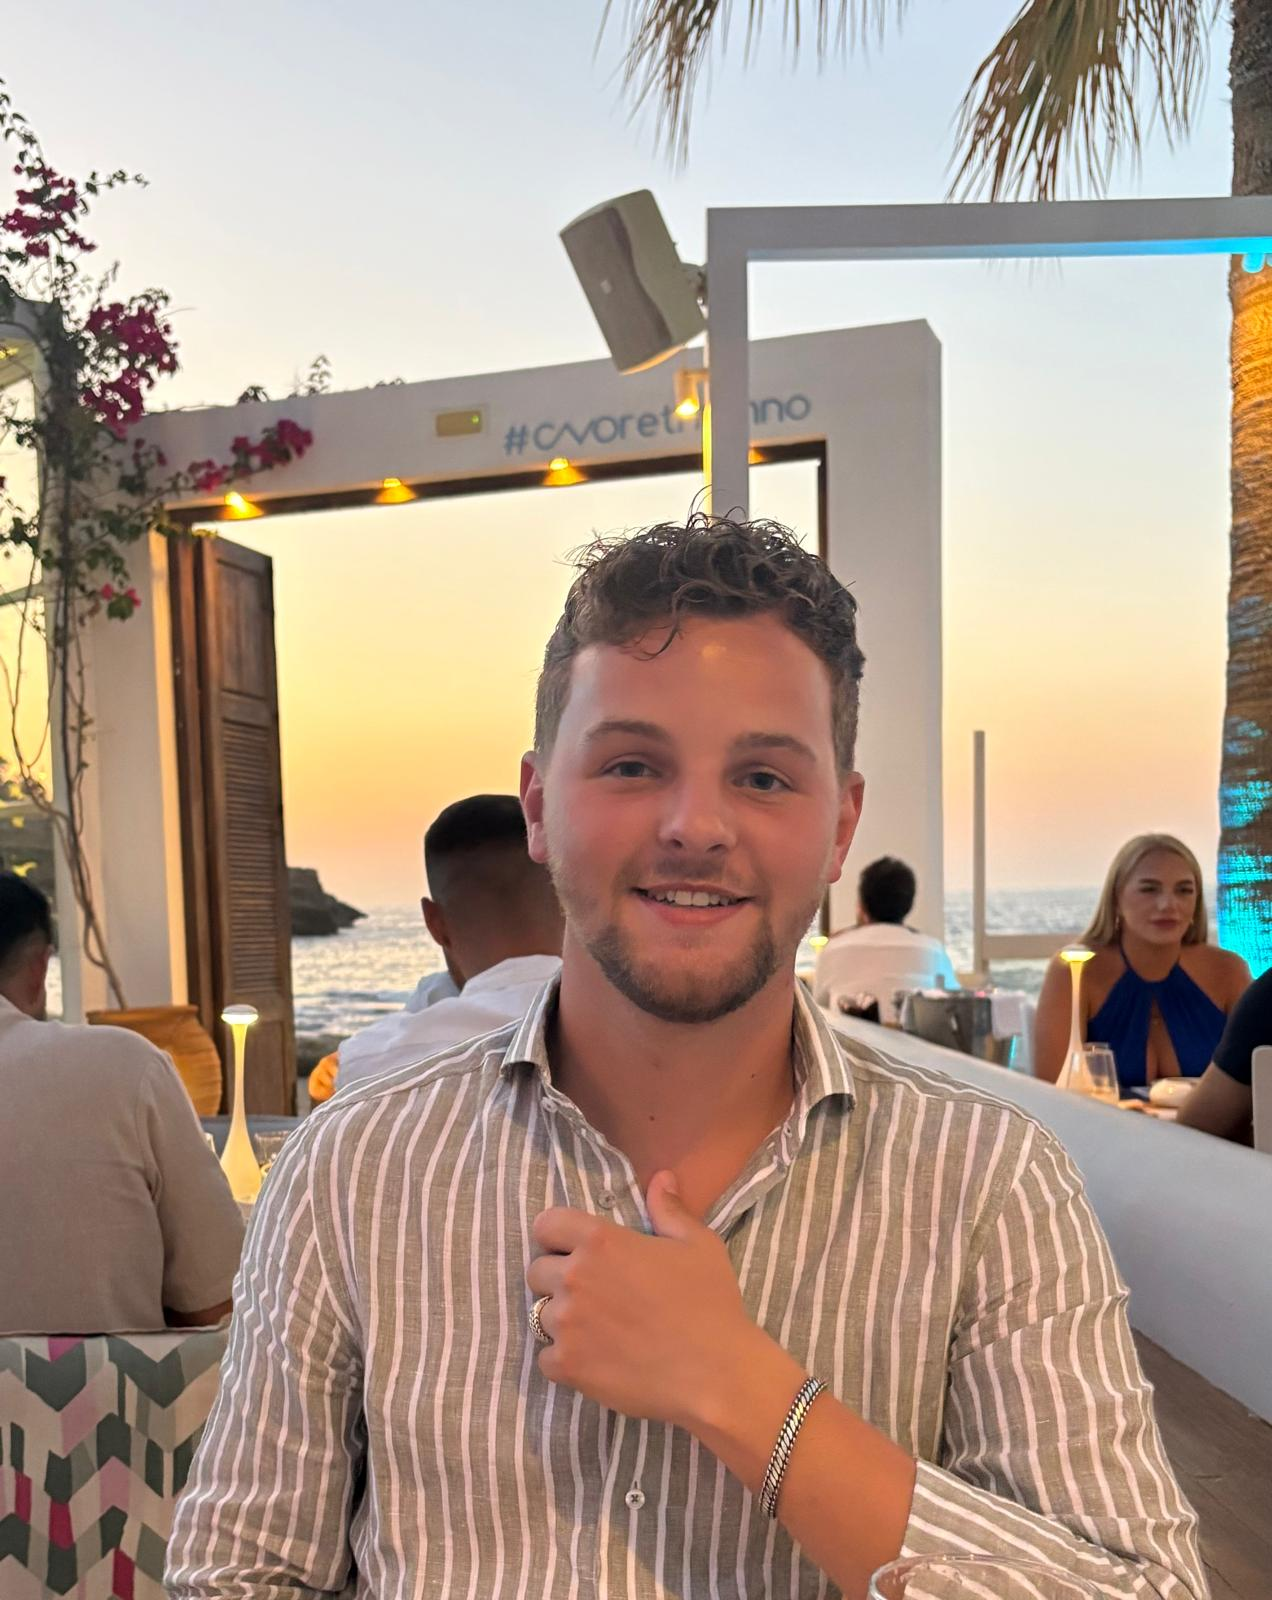
\includegraphics[width=\linewidth]{FotoMarijn.jpg}
\end{minipage}
\hfill
\vspace{1cm}
\begin{minipage}{\linewidth}
	\textbf{Marijn van der Gracht (499194)} \\
	\textbf{Rol:} Voorzitter \\
	Ik ben Marijn van der Gracht, 23 jaar oud en kom uit Hengelo. Ik heb voorafgaand aan de studie BK5, mechatronica gestudeerd aan de Hogeschool Saxion in Enschede. Voor het komende schooljaar vervul ik de rol van Voorzitter in de buitenlandreis commissie. Van mij wordt verwacht dat ik sturing geef aan mijn naaste commissie genoten en communiceer met het bestuur. Ook houd ik rekening met de wensen van de aangesloten studenten bij onze studiereis, zodat iedereen een prettige studiereis heeft. 
\end{minipage}
	
	\newpage
	
	\begin{abstract}
		Dit projectplan beschrijft de voorbereiding, uitvoering en evaluatie van de internationale studiereis van de klas BK5, onderdeel van de opleiding Technische Bedrijfskunde aan Saxion University. De gekozen bestemming is Boedapest, waar zowel culturele als bedrijfskundige elementen centraal zullen staan. Het plan bevat de doelstellingen van de studiereis, een onderbouwing van de gemaakte keuzes en een overzicht van de verwachte leeropbrengsten. Daarnaast worden de betrokken stakeholders en potentiële risico’s in kaart gebracht, evenals de financiële en organisatorische kaders. Ook is een planning opgenomen met de belangrijkste activiteiten en bedrijfsbezoeken, waarmee de reis niet alleen educatief maar ook praktisch waardevol wordt. Dit projectplan dient als leidraad voor alle betrokkenen en vormt de basis voor een gestructureerde en verantwoorde uitvoering van de studiereis naar Boedapest.
	\end{abstract}
	
	\tableofcontents
	
	\newpage
	
	\section{Inleiding}
\IEEEPARstart{D}{it} document vormt het projectplan voor de internationale studiereis van BK5, een klas van de opleiding Technische Bedrijfskunde aan Saxion University. De studiereis is een belangrijk onderdeel van de opleiding, omdat studenten hiermee de mogelijkheid krijgen om in een internationale context kennis en ervaring op te doen, zowel op professioneel als cultureel vlak.

\vspace{0.5cm}

Het doel van dit projectplan is om de voorbereiding en uitvoering van de studiereis gestructureerd vast te leggen en te onderbouwen. Dit is van belang om de leerdoelen van de reis te waarborgen, een duidelijke verdeling van verantwoordelijkheden te creëren en de betrokkenheid van alle stakeholders te borgen.

\vspace{0.5cm}

In dit document worden de doelstellingen en de scope van de studiereis uiteengezet, evenals de gemaakte keuzes ten aanzien van de bestemming en de bijbehorende kosten. Daarnaast worden de betrokken stakeholders geanalyseerd en worden mogelijke risico’s en bijbehorende beheersmaatregelen besproken. Ook bevat het plan een beschrijving van de aanpak en planning, de financiële onderbouwing en het budget, en een communicatieplan waarin de interne en externe informatievoorziening is uitgewerkt.

\vspace{0.5cm}

Tot slot gaat het projectplan in op de evaluatie en verantwoording van de studiereis, zodat achteraf de behaalde resultaten kunnen worden getoetst en verbeterpunten voor toekomstige reizen in kaart gebracht worden. De belangrijkste onderdelen van dit document zijn daarmee als volgt opgebouwd:

\vspace{0.5cm}

\begin{itemize}
	\item \textbf{Doelstelling en scope}
	\item \textbf{Bestemming en programma}
	\item \textbf{Planning en aanpak}
	\item \textbf{Budget en financiën}
	\item \textbf{Risicoanalyse en beheersmaatregelen}
	\item \textbf{Communicatieplan}
	\item \textbf{Evaluatie en verantwoording}
	\item \textbf{Conclusie}
\end{itemize}

\vspace{0.5cm}

Met deze opbouw vormt dit projectplan een gestructureerde leidraad voor de voorbereiding, uitvoering en evaluatie van de studiereis naar Boedapest.
	
	\newpage
	
	\section{Doelstelling en scope}

Dit hoofdstuk definieert de doelstelling en scope van de buitenland reis.

\subsection{Doelstelling}

De internationale studiereis van BK5, opleiding Technische Bedrijfskunde aan Saxion University, heeft als doel studenten en ervaring te laten opdoen in een internationale context. Door het bezoeken van bedrijven in Boedapest of nabijgelegen plaatsen maken studenten kennis met buitenlandse bedrijfsprocessen, managementstructuren en culturele verschillen in ondernemerschap. Naast educatieve waarde wordt met de studiereis ook beoogd de groepsverbinding te versterken door gezamenlijke activiteiten te organiseren die bijdragen aan samenwerking en interculturele vaardigheden.

\vspace{0.5cm}

De studiereis draagt bij aan:

\begin{enumerate}
	\item Het vergroten van de internationale oriëntatie van studenten.
	\item Het opdoen van praktijkervaring door bedrijfsbezoeken en prestaties.
	\item Het stimuleren van samenwerking en teambuilding binnen de klas.
	\item Het verrijken van de studie door het koppelen van theorie aan praktijk in een buitenlandse omgeving.
\end{enumerate}

\subsection{Scope}

De scope van dit projectplan richt zich op de voorbereiding, organisatie en uitvoering van de studiereis naar Boedapest. Dit omvat:

\textbf{Binnen de scope:}

\begin{itemize}
	\item Selectie en bevestiging van de bestemming (Boedapest).
	\item Vastleggen van leerdoelen en educatieve waarde van de reis.
	\item Organisatie van bedrijfsbezoeken in overleg met lokale bedrijven en instellingen.
	\item Ontwikkeling van een programma met zowel educatieve als culturele activiteiten, in samenwerking met de activiteitencommissie.
	\item Financiële planning en begroting, inclusief afstemming met de opleiding en het opstellen van een kostenoverzicht voor studenten.
	\item Logistieke organisatie, zoals vervoer, verblijf en dagplanning.
	\item Communicatie met studenten, begeleiders en stakeholders.
\end{itemize}

\textbf{Buiten de scope:}

\begin{itemize}
	\item Individuele reisarrangementen of persoonlijke uitstapjes buiten het programma.
\end{itemize}
	
	\section{Bestemming en Programma}

Voor de studiereis is in overleg met de klas een poll opgesteld waarin studenten hun voorkeur konden aangeven voor de bestemming. Uit de eerste resultaten kwamen zowel Boedapest als Madrid als populaire opties naar voren (Fig. III.1). Omdat het verschil tussen deze bestemmingen relatief klein was, is er een tweede grafiek gemaakt waarin de eerste en tweede voorkeur staan aangegeven. Uit deze peiling bleek dat Boedapest duidelijk de meeste stemmen kreeg als voorkeursbestemming (Fig. III.2). Op basis van deze uitkomst is besloten de studiereis naar Boedapest (Hongarije) te organiseren.

\begin{figure}[h!]
	\centering
	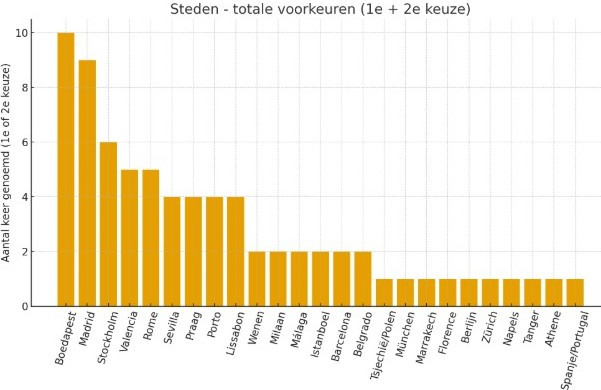
\includegraphics[width=\linewidth]{AllChoices}
	\label{fig:AllChoices}
	\caption{Alle antwoorden van de uitgezette pol.}
\end{figure}

\begin{figure}[h!]
	\centering
	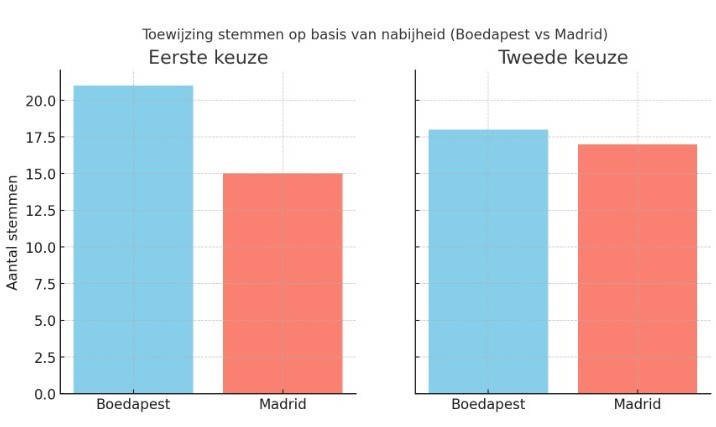
\includegraphics[width=\linewidth]{BudapestVSMadrid}
	\label{fig:MadridVsBoedapest}
	\caption{Boedapest vs Madrid.}
\end{figure}

\newpage

Het programma van de reis is op dit moment nog in ontwikkeling. Aangezien dit projectplan een onderzoeks- en voorbereidingsdocument betreft, worden de definitieve invulling en details van het programma later vastgesteld. De opzet is om het programma samen met de studenten te bepalen door middel van aanvullende polls en door zelf onderzoek te doen naar interessante bedrijven en organisaties in de omgeving van Boedapest. Daarnaast zullen ook culturele en groepsversterkende activiteiten onderdeel uitmaken van het programma, zodat de reis zowel educatief als sociaal waardevol wordt.
	
	\section{Stakeholders}

Voor de organisatie van de internationale studiereis zijn verschillende partijen betrokken. Onderstaand overzicht geeft een stakeholderanalyse weer met daarbij hun invloed en belang bij de reis.

\begin{table}[h!]
	\centering
	\caption{Stakeholderanalyse studiereis BK5}
	\label{tab:stakeholders}
	\begin{tabular}{|l|p{4.5cm}|l|p{4.5cm}|}
		\hline
		\textbf{Stakeholder} & \textbf{Rol / Belang} & \textbf{Invloed / Macht} & \textbf{Communicatie} \\
		\hline
		Projectgroep BK5 (wij) & Organiseren van de studiereis, opstellen planning en budget, contact met bedrijven & Hoog & Regelmatige overleggen, e-mail, projectmeetings \\
		\hline
		Studenten BK5 & Deelnemers van de studiereis, input over voorkeuren en wensen & Gemiddeld & Presentaties, enquêtes, groepsapps \\
		\hline
		Docenten / Begeleiders & Begeleiden van de studiereis, goedkeuring van planning en budget & Hoog & Overleggen, e-mail, voortgangsrapportages \\
		\hline
		Bedrijven & Bezoeken en samenwerking, mogelijk gastcolleges of rondleidingen & Laag tot gemiddeld & E-mailcontact, afspraken voorafgaand aan bezoek, telefonische follow-up \\
		\hline
		Saxion University / School BBT & Formele goedkeuring, verzekeringen, veiligheid & Hoog & Officiële correspondentie, voortgangsrapportages \\
		\hline
	\end{tabular}
	
\end{table}
	
	\newpage
	
	\section{Rolverdeling}
Om de organisatie van de studiereis naar het
buitenland gestructureerd en efficiënt te laten ver
lopen, is er binnen de commissie een duideli
jke taakverdeling opgesteld. Elke functie heeft zijn
eigen verantwoordelijkheden, waardoor er overzicht
en duidelijkheid ontstaat. Onderstaand worden de
verschillende rollen en hun taken toegelicht.

\begin{itemize}
	\item \textbf{Voorzitter} De voorzitter is verantwoordelijk voor de al
	gemene cöordinatie van de commissie. Hij of zij
	bewaakt de voortgang van de voorbereidingen,
	zorgt dat deadlines worden gehaald en dat de
	communicatie tussen de commissieleden goed
	verloopt. Daarnaast vertegenwoordigt de voorzit
	ter de commissie naar buiten toe, bijvoorbeeld
	richting de opleiding en de begeleidende docenten.
	Ook moet de voorzitter aanwezig zijn bij
	alle voorzittersvergaderingen zijn. De voorzitter
	moet iemand zijn die goed overzicht kan houden,
	communicatief sterk is en makkelijk besluiten
	neemt.
	
	\vspace{0.5cm}
	
	\item \textbf{Penningmeester} De penningmeester houdt toezicht op alle financiële zaken rondom de reis. Dit betekent
	het opstellen en beheren van het budget, het
	bijhouden van inkomsten en uitgaven, en het zor
	gen voor een duidelijke financiële verantwoording.
	Ook beheert de penningmeester de betalingen van deelnemers.
	De penningmeester be
	houdt daarnaast nauw contact met de algemene penningmeester van de opleiding die uiteindelijk
	ook het budget van de buitenlandreis beschik
	baar stelt. De penningmeester moet iemand zijn
	die nauwkeurig werkt, goed met cijfers omgaat
	en financieel inzicht heeft.
	
	\item \textbf{Bedrijfscontact} Het commissielid verantwoordelijk voor bedrijf
	scontact onderhoudt de communicatie met de
	bedrijven die tijdens de reis worden bezocht.
	Deze persoon legt het eerste contact, plant af
	spraken in en bevestigt de bezoekmomenten.
	Ook zorgt hij of zij ervoor dat bedrijven tijdig alle
	benodigde informatie ontvangen en dat het programma inhoudelijk aansluit bij de doelen van de
	studiereis. Ook moet er samengewerkt worden
	met de rol logistiek aangezien er vervoer moet
	komen naar het bedrijf. Degene die bedrijfscontact op zich neemt moet iemand zijn die vlot kan
	communiceren, zakelijk correct is en niet bang is
	om bedrijven te benaderen.
	
	\vspace{0.5cm}
	
	\item \textbf{Cöordinator activiteiten \& logistiek} Het commissielid verantwoordelijk voor vervoer
	en activiteiten zorgt voor een goed georgan
	iseerde logistiek en een aantrekkelijk nevenpro
	gramma. Dit houdt in dat hij of zij alle trans
	portzaken regelt, zoals het boeken van de heen
	en terugreis en het lokale vervoer tussen verblijf,
	bedrijven en activiteiten. Deze persoon houdt
	ook nauw contact met de activiteitencommissie
	aangezien zij de activiteiten daadwerkelijk or
	ganiseren. Degene die deze rol op zich neemt
	moet iemand zijn die praktisch ingesteld is, goed
	kan plannen en creatief is in het bedenken van
	activiteiten.
\end{itemize}

Derolverdeling is gedaan op basis van persoonlijke
voorkeuren vooral op basis van wie welke rol het
leukst leek. De verdeling is als volgt opgedeeld:

\begin{table}[h!]
	\centering
	\caption{Takenverdeling commissie BK5 2025-2026}
	\label{tab:takenverdeling}
	\begin{tabular}{|l|l|}
		\hline
		\textbf{Naam} & \textbf{Taak} \\
		\hline
		Marijn van der Gracht & Voorzitter \\
		\hline
		Stijn van Straaten & Penningmeester \\
		\hline
		Tristan van Duuren & Coördinator activiteiten \& logistiek \\
		\hline
		Florent Kegler & Bedrijfscontact \\
		\hline
	\end{tabular}
\end{table}
	
	\section{Communicatie plan}
Het communicatieplan beschrijft hoe wij als projectgroep communiceren met alle betrokken partijen rondom de studiereis. Het doel is dat alle informatie duidelijk, tijdig en gestructureerd wordt gedeeld, zodat de reis soepel verloopt en iedereen goed geïnformeerd is.

\subsection{Communicatie met studenten}
Met de studenten wordt voornamelijk gecommuniceerd over de inhoud van de reis, de dagelijkse planning en praktische zaken. Persoonlijk contact in de klas wordt gebruikt voor aankondigingen en uitleg. Daarnaast worden er digitale flyers via de e-mail verstuurd met belangrijke informatie zoals de bedrijfsbezoeken, tijdsindelingen en locaties. Voorafgaand aan de reis ontvangen de studenten een e-mail met onder andere de kamerindeling, een paklijst en andere praktische informatie. Tijdens de reis kan een whatsapp groep worden gebruikt voor korte vragen en updates.

\subsection{Communicatie met andere commissies en het bestuur}
Voor de afstemming met andere commissies wordt om de twee weken een vergadering georganiseerd met alle voorzitters van de commissies. Deze vergaderingen dienen om de voortgang te bespreken, belangrijke besluiten af te stemmen en om te zorgen dat alle commissies goed samenwerken. Het bestuur en dus de penningmeester is ook bij deze vergaderingen aanwezig, wat belangrijk is om de kosten goed in de gaten te houden. Daarnaast kan e-mail worden gebruikt om extra informatie te delen.

\subsection{Communicatie met bedrijven}
De communicatie met bedrijven waar de bedrijfsbezoeken zullen plaats vinden verloopt voornamelijk via e-mail en telefonisch contact. Hiervoor wordt een nieuw e-mailaccount aangemaakt zodat al het contact op één plek terug te vinden is. Voor directe afspraken of dringende vragen kan er ook telefonisch contact zijn.

\subsection{Communicatie met docenten}
Wij houden de docenten op de hoogte van de voortgang van de studiereis en belangrijke beslissingen. Er kan gecommuniceerd worden via e-mail, in de lessen en tijdens vergaderingen voor toelichting en feedback. Zo wordt ervoor gezorgd dat docenten betrokken zijn en waar nodig ondersteuning kunnen bieden.

\subsection{Onderlinge communicatie binnen de projectgroep}
Binnen de projectgroep wordt samengewerkt met behulp van gezamenlijke documenten voor documentatie, planning en taakverdeling. Op school wordt er overlegt om de voortgang te bespreken, taken te verdelen en beslissingen te nemen. Voor korte vragen, updates en korte communicatie wordt Teams of whatsapp gebruikt.
	
	\section{Kosten en baten}

In dit hoofdstuk wordt een overzicht gepresenteerd van de kosten en begroting van de studiereis voor BK5 in het studiejaar 2025-2026. De tabel geeft inzicht in de uitgaven per student en docent, inclusief accommodatie, vervoer, cultuuractiviteiten en bedrijfsbezoeken. Daarnaast worden eenmalige kosten, zoals bedankjes voor bedrijven en een buffer voor onvoorziene uitgaven, meegenomen. Dit overzicht helpt bij het plannen van de financiële bijdrage van studenten en het bepalen van de benodigde steun vanuit het bestuur of de sponsorcommissie.

\begin{table}[h!]
	\centering
	\caption{Financieel overzicht studiereis BK5 2025-2026}
	\label{tab:financien}
	\begin{tabular}{|l|l|l|l|}
		\hline
		\textbf{Omschrijving} & \textbf{Kosten per student (€)} & \textbf{Kosten per docent (€)} & \textbf{Totaal (€)} \\
		\hline
		Heen- en terugvlucht & 200,00 & 0,00 & 4.400,00 \\
		\hline
		Accommodatie excl. ontbijt & 150,00 & 0,00 & 3.300,00 \\
		\hline
		Accommodatie incl. ontbijt* & 175,00 & 0,00 & 3.850,00 \\
		\hline
		Vervoer van/naar luchthaven & 15,00 & 15,00 & 360,00 \\
		\hline
		Vervoer naar bedrijven en excursies (OV weekkaart) & 20,00 & 20,00 & 480,00 \\
		\hline
		Cultuur/activiteiten & 80,00 & 80,00 & 1.920,00 \\
		\hline
		Uit eten & 50,00 & 50,00 & 1.200,00 \\
		\hline
		Bedrijfsbezoeken** & 15,00 & 15,00 & 360,00 \\
		\hline
		Vervoer naar bedrijfsbezoeken & 25,00 & 25,00 & 575,00 \\
		\hline
		\textbf{Totaal} & 580,00 & 205,00 & 13.170,00 \\
		\hline
		Eenmalige kosten & & & \\
		\hline
		Bedankje bedrijven & 75,00 & & \\
		\hline
		Onvoorziene kosten & 1075,00 & & \\
		\hline
		\textbf{Totaal eenmalige kosten} & & & 575,00 \\
		\hline
		Eigen bijdrage studenten & & & -4.245,00 \\
		\hline
		Eigen bijdrage per student & & & 192,95 \\
		\hline
		De begrote kosten bestuur/sponsorcommissie & & & 9.500,00 \\
		\hline
	\end{tabular}
	
	\vspace{0.5em}
	\footnotesize{* €50 pp voor 7 dagen ontbijt ongeveer €7 per dag. \\
		** €3 pp per bedrijfsbezoek, maximaal €72 per bedrijf.}
\end{table}
	
	\section{Risico's en Maatregelen}

Dit hoofdstuk behandelt de belangrijkste risico’s die tijdens de studiereis kunnen optreden en de maatregelen die genomen kunnen worden om deze te beperken. De risicoanalyse is ingedeeld per categorie, zoals vervoer, verblijf, gezondheid en veiligheid, communicatie en bedrijfsbezoeken. Door vooraf mogelijke problemen in kaart te brengen en preventieve acties te definiëren, kan de reis veilig, soepel en plezierig verlopen voor alle deelnemers en begeleiders.

\begin{table}[h!]
	\centering
	\caption{Risicoanalyse studiereis BK5 2025-2026}
	\label{tab:risicoanalyse}
	\begin{tabular}{|l|p{6cm}|p{5cm}|}
		\hline
		\textbf{Categorie} & \textbf{Risico} & \textbf{Maatregelen / Preventie} \\
		\hline
		Vervoer (vliegen) & Vluchtvertraging of annulering, verlies/beschadiging bagage, groepsleden missen vlucht & Tijdig boeken en bevestigen vluchten, tijdig op luchthaven aanwezig (2–3 uur voor vertrek), zorgen dat iedereen zijn/haar reisverzekering op orde heeft, contactgegevens en reisschema delen met deelnemers \\
		\hline
		Verblijf / accommodatie & Diefstal, ongewenst gedrag van gasten, ontevredenheid/onduidelijkheid over kamerindeling & Hostel/hotel met goede veiligheidsstandaarden kiezen, waardevolle spullen in kluis bewaren, gedragscode bespreken met groep, voorkeuren kamerindeling peilen en vooraf indeling maken \\
		\hline
		Lokaal vervoer & Ongevallen in openbaar vervoer/taxi, deelnemers verdwalen of komen te laat & Heldere afspraken over verzamelpunten/tijden, gebruik betrouwbare taxi’s of openbaar vervoer, telefoonnummers en WhatsApp-groep voor noodgevallen \\
		\hline
		Gezondheid en veiligheid & Ziekte tijdens reis, allergieën, ongevallen & Medische gegevens (bijv. allergieën) vooraf inventariseren, noodnummer(s) verzamelen en delen, reisverzekering inclusief medische dekking \\
		\hline
		Culturele en juridische verschillen & Overtreden lokale wetten, culturele misverstanden & Belangrijkste punten vermelden over lokale wet- en regelgeving, informeren over omgangsvormen en gebruiken \\
		\hline
		Communicatie en coördinatie & Onduidelijkheid in planning, calamiteiten en gedrag, personen vergeten & Centraal aanspreekpunt/reisleider per dag, WhatsApp-groep maken voor het delen van informatie, dagelijkse check-in momentjes (koppen tellen of alternatief), draaiboek maken met alle belangrijke reisinformatie op één plek \\
		\hline
		Bedrijfsbezoeken & Te laat komen, ongepaste kleding of gedrag, ontevredenheid over de bedrijfsbezoeken & Dresscode en gedragsregels vooraf communiceren, programma en adresgegevens vooraf delen, op tijd vertrekken met reismarge, korte briefing per bezoek over cultuur en etiquette, diverse bedrijfssoorten uitkiezen en voorkeuren peilen \\
		\hline
		Alcoholgebruik & Overmatig alcoholgebruik, onder invloed tijdens bedrijfsbezoeken & Vooraf duidelijke gedragsregels opstellen in lijn met de regels vanuit het bestuur, aanspreekpunt aanwijzen, alcoholgebruik vermijden vóór en tijdens zakelijke bezoeken \\
		\hline
	\end{tabular}
\end{table}
	
	\section{Evaluatie en Verantwoording}

De evaluatie en verantwoording van de internationale studiereis zijn essentieel om inzicht te krijgen in de mate waarin de vooraf gestelde doelstellingen zijn gerealiseerd en om te leren voor toekomstige studiereizen. Dit hoofdstuk beschrijft de methoden en instrumenten waarmee de effectiviteit van de reis wordt geëvalueerd en hoe de resultaten worden verantwoord richting de opleiding en overige stakeholders.

\subsection{Evaluatiemethoden}

De evaluatie van de studiereis zal plaatsvinden met behulp van zowel kwantitatieve als kwalitatieve methoden:

\begin{itemize}
	\item \textbf{Enquêtes onder studenten:} direct na de reis ontvangen alle deelnemers een digitale vragenlijst (via tools zoals Google Forms of Mentimeter) waarin zij hun ervaringen, leeropbrengsten en verbeterpunten kunnen aangeven. Hierbij wordt gebruikgemaakt van Likert-schalen om tevredenheid meetbaar te maken, aangevuld met open vragen voor suggesties en tips.
	\item \textbf{Groepsdiscussie:} tijdens een gezamenlijke nabespreking wordt ruimte geboden voor reflectie en het delen van ervaringen. Dit biedt de mogelijkheid om context en nuance te verkrijgen naast de kwantitatieve resultaten.
	\item \textbf{Observaties begeleiders:} de docenten en begeleiders houden tijdens de reis aantekeningen bij over groepsdynamiek, betrokkenheid en organisatorische aandachtspunten.
\end{itemize}

\subsection{Verantwoordingsproces}

De resultaten van de evaluatie worden verwerkt in een \textbf{eindrapport}, waarin onder meer wordt opgenomen:
\begin{itemize}
	\item Een overzicht van de behaalde doelstellingen (SMART getoetst).
	\item De belangrijkste bevindingen uit de enquêtes en groepsdiscussie.
	\item Een vergelijking tussen de geplande doelstellingen en de feitelijke uitvoering.
	\item Aanbevelingen voor toekomstige studiereizen.
\end{itemize}

Dit rapport wordt gedeeld met:
\begin{itemize}
	\item De opleiding Technische Bedrijfskunde (als verantwoordelijke instantie).
	\item De begeleidende docenten.
	\item De activiteitencommissie en de studenten zelf.
\end{itemize}

\subsection{Theoretische onderbouwing}

Volgens de kwaliteitscirkel van Deming (\textit{Plan-Do-Check-Act}) \cite{deming1986out} is de fase van evaluatie en verantwoording cruciaal om continu te verbeteren. Door structureel feedback te verzamelen en terug te koppelen, wordt niet alleen de kwaliteit van toekomstige studiereizen verhoogd, maar ook de verantwoording naar stakeholders geborgd.

\subsection{Tijdsplanning evaluatie}

\begin{itemize}
	\item \textbf{Tijdens de reis:} observaties en korte polls over de organisatie en inhoud van het programma.
	\item \textbf{Direct na terugkomst:} digitale enquête en groepsreflectie.
	\item \textbf{Binnen twee weken na terugkomst:} oplevering van het evaluatierapport en presentatie aan de opleiding.
\end{itemize}
	
	\begin{thebibliography}{00}
		\bibitem{doran1981smart} G. T. Doran, ``There’s a S.M.A.R.T. way to write management’s goals and objectives,'' \textit{Management Review}, vol. 70, no. 11, pp. 35–36, 1981.  
		\bibitem{pmibook2021} Project Management Institute, \textit{A Guide to the Project Management Body of Knowledge (PMBOK Guide)}, 7th ed. Newtown Square, PA: PMI, 2021.
		\bibitem{deming1986out} 
		W. E. Deming, \textit{Out of the Crisis}. Cambridge, MA: MIT Press, 1986.
	\end{thebibliography}
	
\end{document}